\documentclass[letterpaper]{article}
\usepackage{amsmath, amssymb, amsthm}
\usepackage[margin=1in]{geometry}
\usepackage{graphicx}
\usepackage{hyperref}
\usepackage{tikz}
\usepackage{pgfplots}

\title{Flaky Tests in Software Development}
\author{Michael Hering}
\date{\today}
\pgfplotsset{compat=1.18} 

\begin{document}
\maketitle

\begin{abstract}
    TODO use 1/10 fail rate throughout this document
    
    In software development, we use automated test suites to verify the behaviour of our applications. In our CI environments, each commit triggers a build which runs all of the tests and if any of the tests do not pass, the build is failed. This cycle creates rapid feedback which catches failures in our code before going to production and allows us to iterate on our applications with confidence.

    In many test suites, however, we encounter tests that fail sometimes and pass other times even without changes to the application code. These tests, known as "flaky tests", introduce false negatives into the build which significantly increases the feedback loop duration and degrades our confidence in the application behaviour.
    
\end{abstract}


\section{Introduction}

\textbf{Definition:}  A \textit{flaky test} is a test that can pass and fail without changes to the application code under test.

Flaky tests are commonly encountered, even in simple applications. Tests which involve time, concurrency, or any form of asynchronous processing are particularly prone to flakiness and can be difficult to debug.

TODO introduction

---

\section{Analysis}

Here we analyze the relationship between the number of flaky tests and the probability of a successful build, as well as the expected build duration.

\subsection{Single Build Success Probability}

To understand how flaky tests affect the probability of a single build being successful, consider the following:

\setlength{\parskip}{1em}

Let \( n \) be the total number of flaky tests. Assume each flaky test has an independent probability \( p \) of failing on a given run (e.g., \( p = 0.01 \) or 1\%).

For a single flaky test, the probability of passing is \( 1 - p \).

For \( n \) flaky tests, assuming independence, the probability \( P \) that all \( n \) tests pass is:
\[
P = (1 - p)^n.
\]

And as \( n \) grows larger:
\[
\lim_{n \to \infty} (1 - p)^n = 0.
\]

The probability of a single build being successfull decays exponentially with the number of flaky tests.

\subsection{Total Build Duration}
To understand how flaky tests affect total duration required for a successful build, consider the following:

Let \( n \) be the total number of flaky tests. Assume each flaky test has an independent probability \( p \) of failing on a given run (e.g., \( p = 0.01 \) or 1\%).

Let \( t \) be the duration of a single build run (e.g., \( t = 10 \) minutes).

Let \( P \) be the probability that a single build is successfull where \( P = (1 - p)^n \).

If a build fails, it must be re-run to succeed. The expected total time \(T\) to acheive a successfull build follows a geometric distribution:
\[
T = \frac{t}{P} = \frac{t}{(1 - p)^n}.
\]

And as \( n \) grows larger:
\[
\lim_{n \to \infty} T = \infty.
\]

The total build duration grows exponentially with the number of flaky tests. 


\subsection{Numerical Examples}

Consider the following examples:

 Let \( p = 0.1 \) where \(p\) is the probability of a single flaky test failing on a given run.

 Let \( t = 10 \) minutes where \(t\) is the duration of a single successful build.

 Let \(S\) be the probability that the build is successfull where \(S = (1 - p)^n\).

 Let \(N\) be the average expected number of runs to achieve a successful build where \(N = \frac{1}{S}\).

 Let \(T\) be the average expected total build duration to achieve a successful build where \(T = t \times N\).


\textbf{1 Flaky Test:}
\[
S = 0.9, \quad N \approx 1.11, \quad T \approx 11.1 \text{ minutes}.
\]

\textbf{4 Flaky Tests:}
\[
S = 0.9^{4} \approx 0.656, \quad N \approx 1.52, \quad T \approx 15.2 \text{ minutes}.
\]

\textbf{16 Flaky Tests:}
\[
S = 0.9^{16} \approx 0.185, \quad N \approx 5.40, \quad T \approx 54.0 \text{ minutes}.
\]

\textbf{64 Flaky Tests:}
\[
S = 0.9^{64} \approx 0.001, \quad N \approx 841.6, \quad T \approx 8,481.6 \text{ minutes}.
\]

\pagebreak

\begin{figure}[h!]
    \centering
    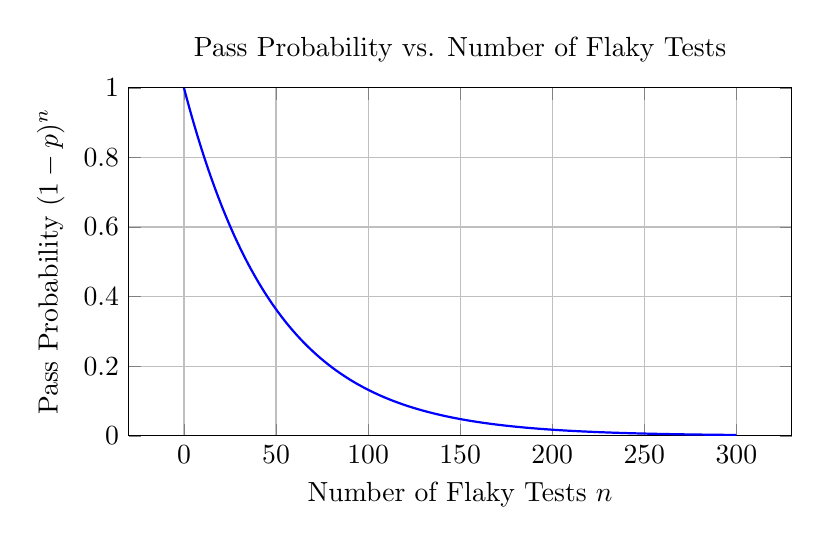
\begin{tikzpicture}
    \begin{axis}[
        title={Pass Probability vs. Number of Flaky Tests},
        ylabel={Pass Probability $(1-p)^n$},
        xlabel={Number of Flaky Tests $n$},
        ymin=0, ymax=1,
        domain=0:300,
        samples=200,
        width=10cm,
        height=6cm,
        grid=major
    ]
    \addplot[blue, thick] { (1-0.02)^x };
    \end{axis}
    \end{tikzpicture}
    \caption{As $n$ grows, $(1-p)^n$ declines sharply from 1 to near 0. For $p=0.01$, the probability of a completely passing build becomes very small as $n$ increases.}
\end{figure}

\begin{figure}[h!]
    \centering
    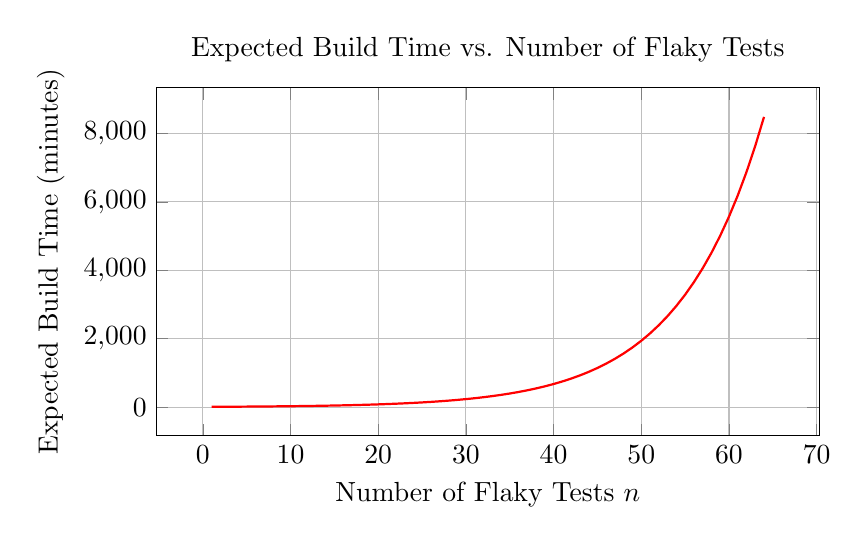
\begin{tikzpicture}
    \begin{axis}[
        title={Expected Build Time vs. Number of Flaky Tests},
        ylabel={Expected Build Time (minutes)},
        xlabel={Number of Flaky Tests $n$},
        domain=1:64,
        samples=64,
        width=10cm,
        height=6cm,
        grid=major
    ]
    \addplot[red, thick] {10/(0.9^x)};
    \end{axis}
    \end{tikzpicture}
    \caption{Expected build time grows exponentially with the number of flaky tests.}
\end{figure}


These examples illustrate how the expected number of builds and total build duration increases significantly with the number of flaky tests.



\section*{Marginal Impact of Fixing Individual Tests}

TODO It's not all bad though!!! 

When a flaky test is fixed, the improvement in pass probability depends greatly on how many flaky tests remain. Consider fixing one flaky test in different scenarios, where each test has $p=0.1$ failure rate:

\begin{itemize}
    \item Going from 64 to 63 flaky tests: Pass rate improves from 0.001 to 0.001 (0.01\%)
    \item Going from 16 to 15 flaky tests: Pass rate improves from 0.185 to 0.206 (2.1\%)
    \item Going from 4 to 3 flaky tests: Pass rate improves from 0.656 to 0.729 (7.3\%)
    \item Going from 1 to 0 flaky tests: Pass rate improves from 0.900 to 1.000 (10.0\%)
\end{itemize}

This demonstrates that fixing flaky tests has increasing marginal returns. As you move from right to left the impact of each fix becomes more significant as the total count decreases.

\begin{figure}[h!]
    \centering
    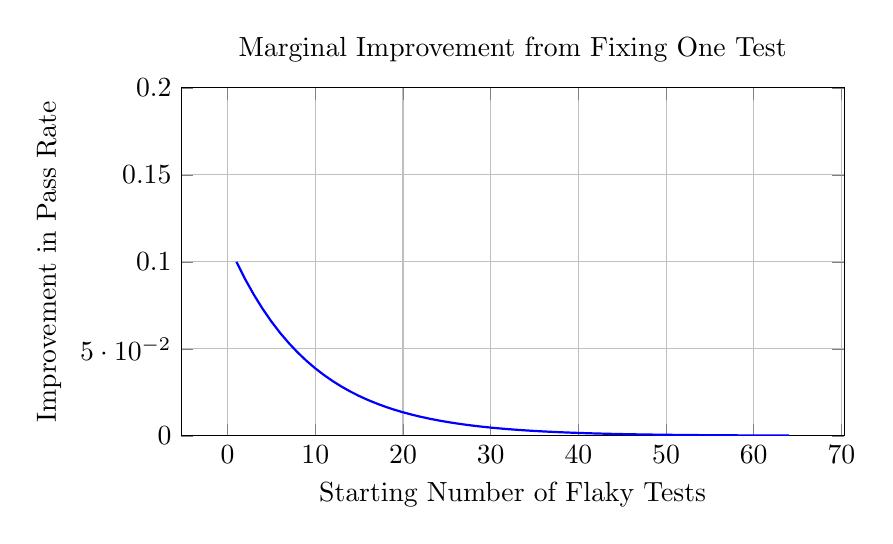
\begin{tikzpicture}
    \begin{axis}[
        title={Marginal Improvement from Fixing One Test},
        ylabel={Improvement in Pass Rate},
        xlabel={Starting Number of Flaky Tests},
        ymin=0, ymax=0.2,
        domain=1:64,
        samples=64,
        width=10cm,
        height=6cm,
        grid=major
    ]
    \addplot[blue, thick] {(0.9^(x-1))-(0.9^x)};
    \end{axis}
    \end{tikzpicture}
    \caption{The marginal improvement in pass rate when fixing one test, starting from $n$ tests.}
\end{figure}

\section*{Conclusion}

TODO some more about why we care

Flaky tests create a compounding effect: even a small failure rate per test can lead to a near-certain failure when combined. This results not only in failing CI builds but also in an exponential increase in the expected time to achieve a clean, passing build. The necessity of re-runs consumes additional minutes, slowing development cycles and delaying feedback.

The flip side is that by maintaining a healthy build environment, you minimize both the probability of failures and the wasted time associated with re-runs. The sooner you address flaky tests—the moment one appears—the less cumulative effort you pay later. It is far more efficient to fix them now rather than waiting until there are 20 flaky tests that must be fixed all at once. A timely fix preserves a stable CI pipeline and keeps development running smoothly.

TODO a small comment because sometimes you have do what you have to do and take on some debt....  so, fix them now - or don't right now, but very very soon.

\end{document}
